% id: 96-46
% book: 쎈B 대수 · 07 삼각함수의 활용
% section: 유형 11 삼각형의 넓이
% figure: tikz:fig-96-46
% answer: 
% answer_source: 
% variant_level: 0 (원본 전사)
% 이 파일은 build.mjs 가 items.json 에서 만든다. 고칠 때는 items.json 을 고친다.
\noindent\begin{minipage}[t]{0.58\linewidth}\vspace{0pt}\raggedright 오른쪽 그림과 같이 $\seg{AB}=4$, $\seg{BC}=\sqrt{26}$, $\seg{AD}\cdot\seg{CD}=30$이고 $\angle\pt{BAC}=\dfrac{\pi}{4}$인 사각형~$\pt{ABCD}$가 있다. 삼각형~$\pt{ABC}$의 넓이를 $S_1$, 삼각형~$\pt{ACD}$의 넓이를 $S_2$라 하면 $S_2=\dfrac{6}{5}S_1$일 때, 삼각형~$\pt{ACD}$의 외접원의 반지름의 길이를 구하시오.\end{minipage}\hfill\begin{minipage}[t]{0.4\linewidth}\vspace{0pt}\centering \resizebox{\ifdim\width>\linewidth\linewidth\else\width\fi}{!}{% 96-46(96쪽) — 사각형 ABCD 와 세 점 A·C·D 를 지나는 원(원문 「오른쪽 그림」 · 점 B 는 원 밖). 스캔 화질이 낮아 TikZ 로 다시 그림.
% 라벨은 원문 것만: 꼭짓점 A·B·C·D, 길이 4·$\sqrt{26}$, $\angle\pt{BAC}=\dfrac{\pi}{4}$. 길이 표시의 점선 호는 원문 꼴.
% 외접원의 반지름(답)이 읽히지 않게 중심·반지름은 그리지 않는다.
\begin{tikzpicture}[line width=0.6pt, x=1cm, y=1cm, >=stealth]
  \coordinate (A) at (-1.549,0.054);
  \coordinate (D) at (-1.025,1.164);
  \coordinate (C) at (0.621,-1.421);
  \coordinate (B) at (-1.271,-1.404);
  \draw (0,0) circle (1.55);
  \draw (A) -- (B) -- (C) -- (D) -- cycle;
  \draw[line width=0.45pt] (A) -- (C);
  % $\angle\pt{BAC}$ 표시
  \draw[line width=0.4pt] ([shift=(-79.2:0.40)]A) arc (-79.2:-34.2:0.40);
  \node[font=\footnotesize] at (-0.72,0.14) {$\dfrac{\pi}{4}$};
  \draw[->, line width=0.35pt] (-0.98,-0.06) to[bend left=15] (-1.27,-0.36);
  % 길이 표시의 점선 호
  \draw[densely dashed, line width=0.35pt] (A) to[bend right=20] (B);
  \draw[densely dashed, line width=0.35pt] (B) to[bend right=20] (C);
  \node[font=\small] at (-1.80,-0.60) {$4$};
  \node[font=\small] at (-0.32,-1.86) {$\sqrt{26}$};
  \node[font=\small, anchor=east] at (-1.62,0.10) {$\pt{A}$};
  \node[font=\small, anchor=south east] at (-1.07,1.22) {$\pt{D}$};
  \node[font=\small, anchor=west] at (0.70,-1.45) {$\pt{C}$};
  \node[font=\small, anchor=east] at (-1.34,-1.44) {$\pt{B}$};
\end{tikzpicture}
}\end{minipage}\par
